\begin{figure}
    \centering
    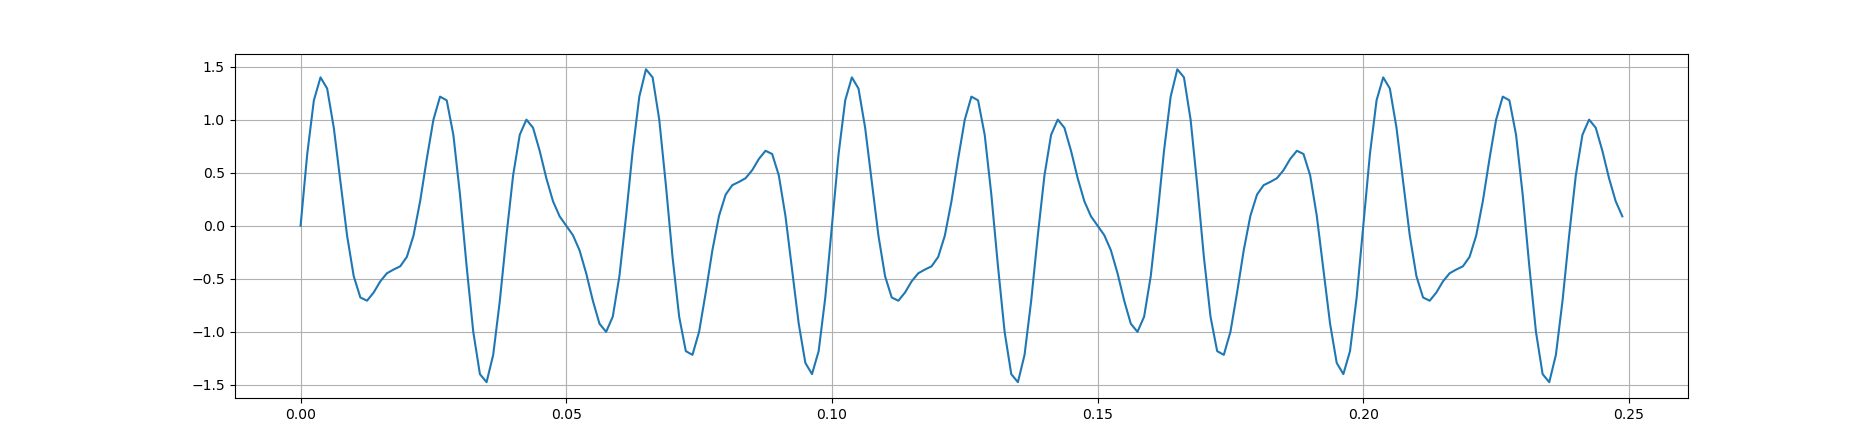
\includegraphics[scale=0.2]{figures/FourierTransform.png}
    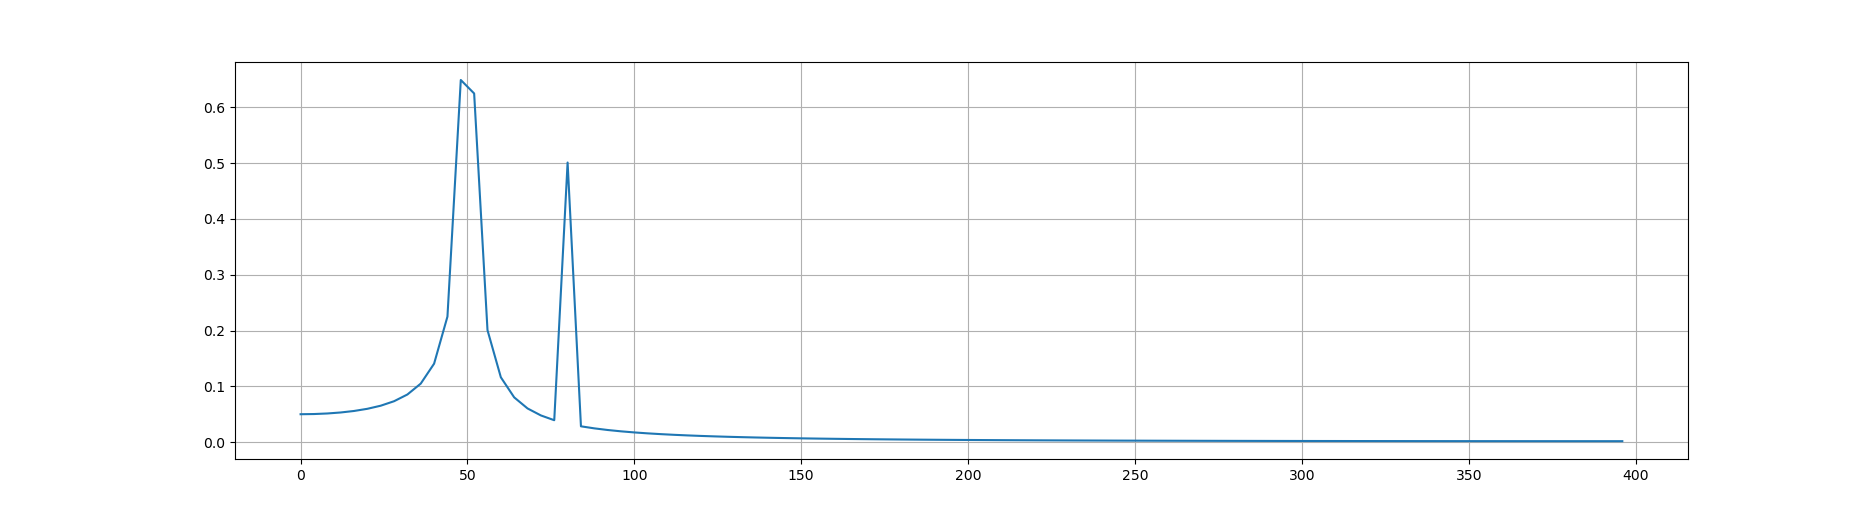
\includegraphics[scale=0.2]{figures/FourierTransformed.png}
    \caption{Fast Fourier Transform as an example through transforming the top signal in to representation in the frequency domain at the bottom.}
    \label{fig:fft}
\end{figure}

% automatically generated by the script in the /music_recognition_main/figure_generation/arraydiagram.py
\begin{figure}
    \centering
    \begin{tikzpicture}
    \matrix (m) [table]
    {
 |[fill=6]| & |[fill=15]| & |[fill=8]| & |[fill=11]| & |[fill=6]| \\
 |[fill=10]| & |[fill=10]| & |[fill=6]| & |[fill=1]| & |[fill=14]| \\
 |[fill=13]| & |[fill=2]| & |[fill=7]| & |[fill=7]| & |[fill=1]| \\
 |[fill=3]| & |[fill=6]| & |[fill=9]| & |[fill=9]| & |[fill=5]| \\
 |[fill=9]| & |[fill=2]| & |[fill=15]| & |[fill=11]| & |[fill=3]| \\
 |[fill=11]| & |[fill=10]| & |[fill=4]| & |[fill=12]| & |[fill=3]| \\
    };
    \matrix (mat) [table, right=2.5cm of m]
    {
 |[fill=6]| & |[fill=15]| & |[fill=8]| & |[fill=11]| & |[fill=6]| \\
 |[fill=10]| & |[fill=10]| & |[fill=6]| & |[fill=1]| & |[fill=14]| \\
 |[fill=13]| & |[fill=2]| & |[fill=7]| & |[fill=7]| & |[fill=1]| \\
 |[fill=3]| & |[fill=6]| & |[fill=9]| & |[fill=9]| & |[fill=5]| \\
 |[fill=9]| & |[fill=2]| & |[fill=15]| & |[fill=11]| & |[fill=3]| \\
 |[fill=11]| & |[fill=10]| & |[fill=4]| & |[fill=12]| & |[fill=3]| \\
    };
        \node [above=3pt of m-1-3] (test) {\textcolor{Red}{Time (Second)}};
        \node [above=3pt of mat-1-3] (test) {\textcolor{Red}{Time (Second)}};
        \node [left=3pt of mat-3-1] (test) {\textcolor{Blue}{Frequency (Hz)}};

        \draw [blue,thick] plot[only marks,mark=x,mark size=6pt] (mat-1-1); 
        \draw [blue,thick] plot[only marks,mark=x,mark size=6pt] (mat-1-2); 
        \draw [blue,thick] plot[only marks,mark=x,mark size=6pt] (mat-1-4); 
        \draw [blue,thick] plot[only marks,mark=x,mark size=6pt] (mat-2-1); 
        \draw [blue,thick] plot[only marks,mark=x,mark size=6pt] (mat-2-5); 
        \draw [blue,thick] plot[only marks,mark=x,mark size=6pt] (mat-3-1); 
        \draw [blue,thick] plot[only marks,mark=x,mark size=6pt] (mat-3-4); 
        \draw [blue,thick] plot[only marks,mark=x,mark size=6pt] (mat-4-3); 
        \draw [blue,thick] plot[only marks,mark=x,mark size=6pt] (mat-4-4); 
        \draw [blue,thick] plot[only marks,mark=x,mark size=6pt] (mat-5-1); 
        \draw [blue,thick] plot[only marks,mark=x,mark size=6pt] (mat-5-3); 
        \draw [blue,thick] plot[only marks,mark=x,mark size=6pt] (mat-6-1); 
    \end{tikzpicture}
    \caption{Illustrating the picking of points, the darker the box, the darker the amplitude (value) represents}
    \label{fig:listfiltering}
\end{figure}


\begin{figure}
    \centering
    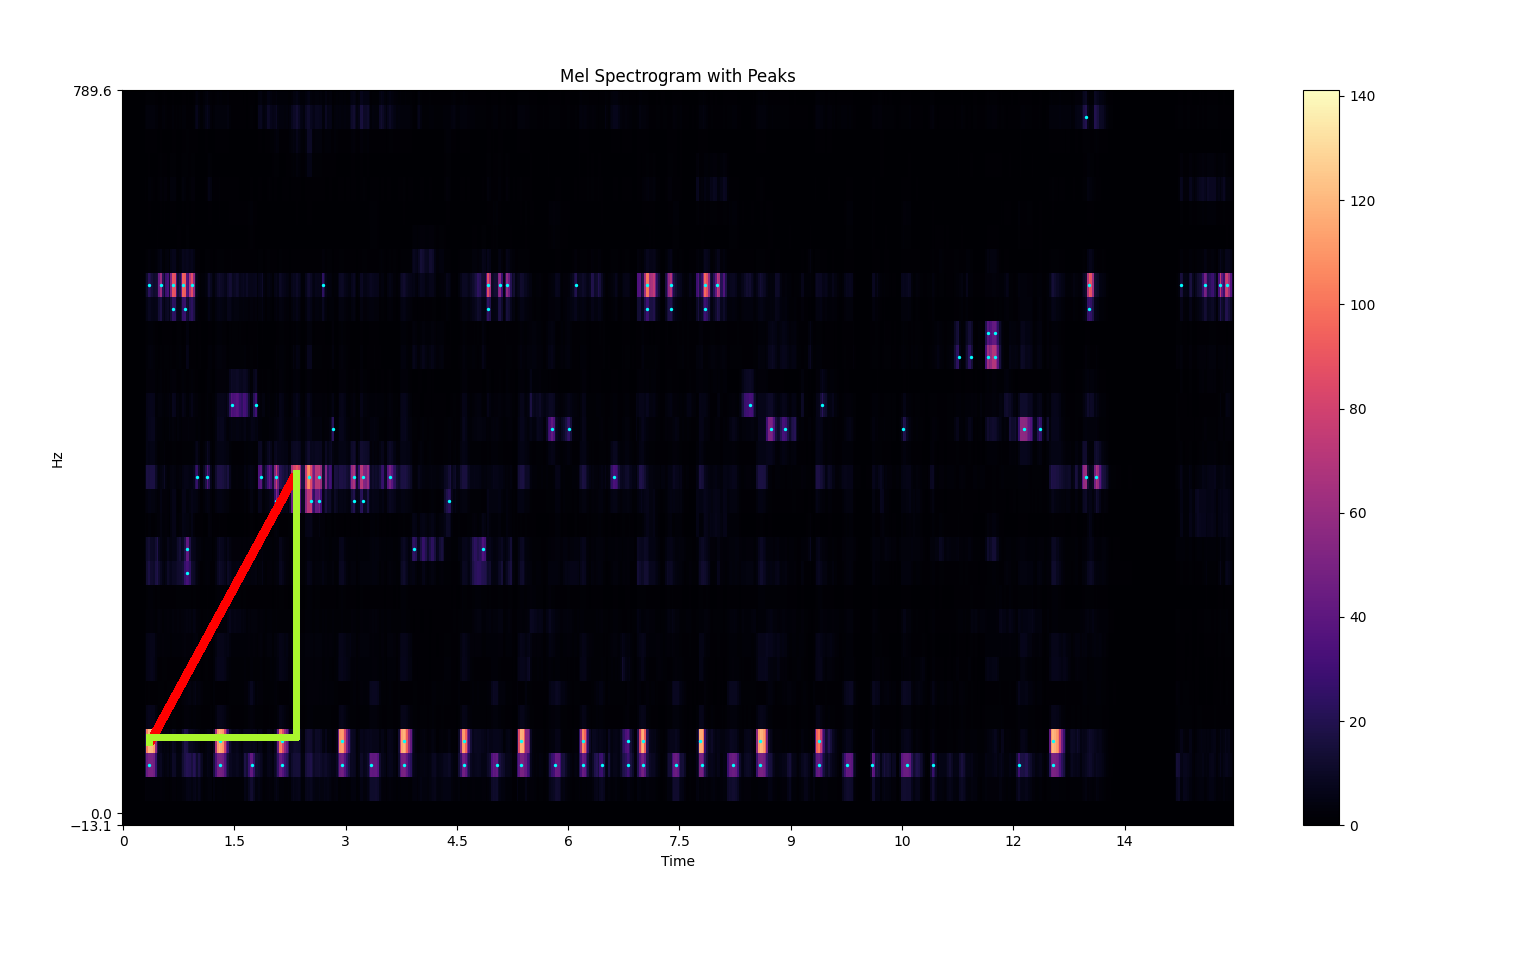
\includegraphics[scale=0.2]{figures/Delta_distance_demo.png}
    \caption{The tip of the triangle represents Point A and Point B. Y-axis represents the time, X-axis represents the frequency, The amplitude scales are represented by the colour bar on the right.}
    \label{fig:pairspicking}
\end{figure}

\begin{figure}
    \centering
    \small
        \begin{tabular}{|c|c|c|c|c|}
            \hline
            Point A (Hz) & Point B (Hz) & Time delta (s) & Point A time (s) & Track UUID \\
            \hline
            20.1 & 302.1 & 1.8 & 0.3 & $ea47a3c5$\\
            \hline
            \multicolumn{3}{|c|}{$2388532207457024332$} & 2.1 & $ea47a3c5$\\
            \hline
        \end{tabular}
    \caption{Demonstrate / example of how item are hashed. \cite{macleod_abracadabra_nodate}}
    \label{fig:hash}
\end{figure}


\begin{figure}
    \centering
    \begin{tabular}{|c|c|c|c|}
        \hline
        Song\_ID & Name & Author & Genre \\
        \hline
        f633c47a & J. S. Bach: Prelude in C - BWV 846  & Kevin MacLeod & Classical \\
        \hline
    \end{tabular}
    \caption{Example of a database entry}
    \label{fig:database}
\end{figure}
